%\documentclass[border=10pt]{standalone}
%\usepackage{tikz}
\tikzset{
	treenode/.style = {shape=rectangle, rounded corners,
		draw, align=center,
		top color=white, bottom color=blue!20},
	root/.style     = {treenode, font=\ttfamily\normalsize},
	env/.style      = {treenode, font=\ttfamily\normalsize},
	dummy/.style    = {circle,draw},
	level 1/.style={sibling distance=6cm, level distance = 3em},
	level 2/.style={sibling distance=2.5cm,level distance = 5em}, 
	level 3/.style={sibling distance=2cm},
	blueRed/.style={env, top color=blue, bottom color=red} 
}
%\begin{document}
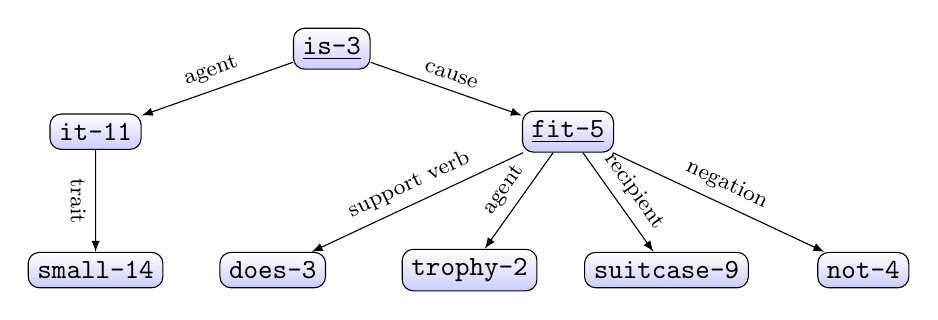
\begin{tikzpicture}
[
grow                    = down,
sibling distance        = 50em,
level distance          = 5em,
edge from parent/.style = {draw, -latex},
every node/.style       = {font=\footnotesize},
sloped
]
\node [root] {\underline{is-3}}
child { node [env ] {\textbf{it-11}}
	child {node [env] {\textbf{small-14}}
		edge from parent node [below] {trait} }
	edge from parent node [above] {agent}}
child { node [env] {\underline{fit-5}}
	child {node [env]  {\textbf{does-3}}
		edge from parent node [above] {support verb} }	
	child {node [env ]  {\textbf{trophy-2}}
		edge from parent node [above] {agent} }
	child {node [env ]  {\textbf{suitcase-9}}
		edge from parent node [above] {recipient}}
	child {node [env]  {\textbf{not-4}}
		edge from parent node [above] {negation} }
	edge from parent node [above] {cause}};

\end{tikzpicture}
%\end{document}